% ============================================================
%  DeepFakeDetector — Research Paper
%  McMaster AI Society
%  Compile with: pdflatex -> bibtex -> pdflatex -> pdflatex
% ============================================================

\documentclass[12pt, a4paper]{article}

% ---- Core packages ----
\usepackage[margin=1in]{geometry}
\usepackage{amsmath, amssymb, amsthm}
\usepackage{graphicx}
\usepackage{booktabs}
\usepackage{multirow}
\usepackage{array}
\usepackage[hidelinks, colorlinks=false]{hyperref}
\usepackage{xcolor}
\usepackage{caption}
\usepackage{subcaption}
\usepackage{float}
\usepackage{enumitem}
\usepackage{microtype}
\usepackage{setspace}
\usepackage{fancyhdr}
\usepackage{authblk}
\usepackage{titlesec}

% ---- TikZ (architecture diagram) ----
\usepackage{tikz}
\usetikzlibrary{shapes.geometric, arrows.meta, positioning, fit, calc, backgrounds}

% ---- Bibliography ----
\usepackage[numbers, sort&compress]{natbib}

% ---- PGFPlots (training curves) ----
\usepackage{pgfplots}
\pgfplotsset{compat=1.18}

% ================================================================
%  Custom colours
% ================================================================
\definecolor{mcmaster}{RGB}{122, 0, 20}
\definecolor{nodeblue}{RGB}{31, 119, 180}
\definecolor{nodegreen}{RGB}{44, 160, 44}
\definecolor{nodered}{RGB}{214, 39, 40}
\definecolor{nodeorange}{RGB}{255, 127, 14}
\definecolor{nodegray}{RGB}{127, 127, 127}
\definecolor{lightgray}{RGB}{245, 245, 245}

% ================================================================
%  TikZ node styles
% ================================================================
\tikzset{
  inputnode/.style={
    rectangle, rounded corners=4pt,
    minimum width=3.2cm, minimum height=0.75cm,
    text centered, font=\small\bfseries,
    draw=mcmaster, fill=mcmaster!10, thick
  },
  preprocnode/.style={
    rectangle, rounded corners=4pt,
    minimum width=9cm, minimum height=0.75cm,
    text centered, font=\small,
    draw=nodeblue, fill=nodeblue!10, thick
  },
  modelnode/.style={
    rectangle, rounded corners=4pt,
    minimum width=2.4cm, minimum height=1.4cm,
    text centered, font=\scriptsize,
    draw=nodegreen, fill=nodegreen!10, thick
  },
  embnode/.style={
    rectangle, rounded corners=2pt,
    minimum width=2.1cm, minimum height=0.6cm,
    text centered, font=\scriptsize,
    draw=nodegray, fill=lightgray, thick
  },
  fusionnode/.style={
    rectangle, rounded corners=4pt,
    minimum width=5.5cm, minimum height=0.75cm,
    text centered, font=\small,
    draw=nodered, fill=nodered!10, thick
  },
  outputnode/.style={
    rectangle, rounded corners=4pt,
    minimum width=4.2cm, minimum height=0.75cm,
    text centered, font=\small\bfseries,
    draw=nodeorange, fill=nodeorange!10, thick
  },
  myarrow/.style={thick, ->, >=Stealth, color=gray!70}
}

% ================================================================
%  Page style
% ================================================================
\pagestyle{fancy}
\fancyhf{}
\lhead{\textcolor{mcmaster}{\textbf{McMaster AI Society}}}
\rhead{DeepFakeDetector}
\cfoot{\thepage}
\renewcommand{\headrulewidth}{0.4pt}

\onehalfspacing
\setlength{\parindent}{1.5em}
\setlength{\parskip}{0.3em}

% ================================================================
%  Title
% ================================================================
\title{
  \vspace{-0.8cm}
  {\color{mcmaster}\rule{\linewidth}{2pt}}\\[0.5em]
  \textbf{DeepFakeDetector: A Multi-Branch Fusion Framework\\
    for Cross-Generator Detection of AI-Generated Images}\\[0.4em]
  {\color{mcmaster}\rule{\linewidth}{1pt}}\\[0.3em]
  \large McMaster AI Society — Technical Report
}

\author[1]{McMaster AI Society}
\affil[1]{%
  Department of Electrical \& Computer Engineering,
  McMaster University, Hamilton, Ontario, Canada
}
\date{February 2026}

% ================================================================
\begin{document}
% ================================================================

\maketitle
\thispagestyle{fancy}

% ================================================================
\begin{abstract}
\noindent
The rapid proliferation of AI-generated imagery produced by generative
adversarial networks (GANs) and latent diffusion models presents a mounting
challenge for digital media authenticity.  Existing detection systems frequently
overfit to generators seen during training, failing catastrophically on novel
architectures.  We introduce \textit{DeepFakeDetector}, a multi-branch fusion
framework designed for cross-generator generalisation that combines four
complementary detection modalities: \textbf{(1)}~a fine-tuned Vision Transformer
(ViT-Base/16) operating on RGB patches; \textbf{(2)}~a knowledge-distilled
DeiT-Base model for CPU-efficient inference; \textbf{(3)}~a compact
frequency-domain CNN (CompactFFTNet, $\approx$50\,K parameters) analysing
log-magnitude FFT spectra; and \textbf{(4)}~a five-channel Gradient Field CNN
exploiting spatial coherence derived from the image structure tensor.  Individual
branch accuracies range from 72.69\% (frozen ViT) to 97.05\% (Gradient Field
CNN), with the gradient branch achieving perfect specificity (0 false positives
on 1\,000 real test images).  Branches are fused via a feature-level meta-MLP
(2048-D concatenated embeddings $\rightarrow$ 512 $\rightarrow$ 128 $\rightarrow$
1, $\approx$1.3\,M parameters), targeting AUROC $>$ 0.92 and accuracy $>$ 89\%
on unseen generators.  Total GPU inference latency is $\approx$93\,ms, satisfying
interactive web-application requirements ($\leq$150\,ms).
\end{abstract}

\noindent\textbf{Keywords:} deepfake detection, AI-generated image forensics,
vision transformer, frequency domain, gradient field coherence, multi-branch
fusion, cross-generator generalisation.

\vspace{0.5em}
\noindent{\color{mcmaster}\rule{\linewidth}{0.8pt}}

% ================================================================
\section{Introduction}
\label{sec:intro}

\subsection{Motivation}

The democratisation of generative AI has dramatically lowered the barrier to
creating photorealistic synthetic imagery.  Text-to-image diffusion models —
Stable Diffusion, DALL·E 3, Midjourney, Flux — can produce near-imperceptible
fakes in seconds, while face-swapping tools powered by autoencoders and GANs
enable manipulation of video footage with equally alarming fidelity.  The social
consequences include misinformation campaigns, non-consensual synthetic media,
erosion of evidentiary trust, and financial fraud.

Automated detection is therefore an urgent technical priority.  Yet detection is
fundamentally a moving target: each new generative architecture introduces novel
artifact distributions, and detectors trained exclusively on known generators
exhibit steep performance degradation on unseen ones.  A practical detection
system must generalise beyond its training distribution, operate at interactive
web speeds, and be transparent enough to earn user trust.

The DeepFakeDetector project, developed by the McMaster AI Society, addresses
these requirements through a multi-branch architecture that exploits
complementary signals: global semantic consistency (ViT/DeiT via self-attention
over image patches), frequency-domain spectral fingerprints (CompactFFTNet via
log-magnitude FFT), and structural edge coherence (Gradient Field CNN via
structure-tensor eigenanalysis).  A learned fusion module aggregates branch
embeddings into a calibrated probability estimate.

\subsection{Related Works}
\label{sec:related}

\textbf{Supervised CNN baselines.}
Wang et al.~\cite{wang2020cnn} demonstrated that CNNs trained on ProGAN-generated
images generalise surprisingly well to other GAN architectures.  However,
generalisation to diffusion models — which carry fundamentally different spectral
signatures — remains limited.

\textbf{Feature-probing on foundation models (UnivFD).}
Ojha et al.~\cite{ojha2023univfd} froze a CLIP ViT backbone and trained only a
linear probe on its features, achieving strong cross-generator generalisation.
Their key insight — that large-scale vision pretraining produces representations
that natively separate real and synthetic images — directly informs our ViT and
DeiT branches.

\textbf{Diffusion-domain reconstruction (DIRE).}
Wang et al.~\cite{wang2023dire} proposed computing the reconstruction error when
re-encoding an image through a diffusion model: synthetic images lie near the
model's learned manifold and reconstruct with high fidelity, while real photos
do not.  DIRE achieves very strong cross-generator results but incurs 10–50$\times$
the latency of a single forward pass, making it unsuitable as a primary
interactive detector.

\textbf{Patch-based artifact detection (SSP/ESSP).}
Li et al.~\cite{li2024ssp} (Simple Patch Selection) focused detection on
low-texture regions — sky, walls, smooth surfaces — where generative models leave
characteristic statistical residuals.  This approach provides excellent
explainability (users can see exactly which patch triggered the alert) but
degrades under JPEG compression, which ESSP partially addresses.

\textbf{Frequency-domain methods.}
Generative models leave characteristic fingerprints in the frequency domain: GANs
exhibit periodic artifacts in high-frequency components, and diffusion denoisers
produce distinctive spectral energy distributions~\cite{corvi2023intriguing}.
Frequency-aware dual-path architectures consistently outperform purely spatial
baselines on face-specific deepfake datasets.

\textbf{Face-specific deepfake detection.}
FaceForensics++~\cite{rossler2019faceforensics} standardised evaluation on
face-region video manipulation.  Celeb-DF~\cite{li2020celebdf} demonstrated that
models trained on FaceForensics++ fail dramatically on the more realistic
Celeb-DF benchmark, underscoring the generalisation problem.  Our work targets
general images rather than face-specific manipulation.

Table~\ref{tab:related_comparison} summarises the key approaches.

\begin{table}[H]
\centering
\caption{Comparison of deepfake detection approaches relevant to this work.}
\label{tab:related_comparison}
\resizebox{\textwidth}{!}{%
\begin{tabular}{llllll}
\toprule
\textbf{Approach} & \textbf{Open Source} & \textbf{Inference Speed}
  & \textbf{Cross-Gen.} & \textbf{Compression Robust.} & \textbf{Explainability} \\
\midrule
UnivFD (CLIP/ViT probe) \cite{ojha2023univfd}
  & Yes & Fast & \textbf{Strong} & Good & Attention maps \\
SSP / ESSP \cite{li2024ssp}
  & SSP: Yes & Very fast & Moderate & SSP: Weak & \textbf{Excellent} \\
Frequency CNN (various)
  & Yes & Fast–Med & Good & \textbf{Excellent} & Moderate \\
DIRE (diffusion recon.) \cite{wang2023dire}
  & Yes & \textbf{Slow (10–50$\times$)} & \textbf{Very strong} & Excellent & Moderate \\
Plain CNN baseline \cite{wang2020cnn}
  & Yes & Fast & Weak–Moderate & Fair & Basic \\
\textbf{Ours (multi-branch fusion)}
  & Yes & $\approx$93\,ms GPU & TBD (cross-gen eval.) & TBD & Planned \\
\bottomrule
\end{tabular}%
}
\end{table}

\subsection{Problem Definition}
\label{sec:problem}

Let $\mathcal{X} = \{(x_i, y_i)\}_{i=1}^{N}$ denote a dataset of images
$x_i \in \mathbb{R}^{H \times W \times 3}$ with binary labels $y_i \in \{0,1\}$
where $y_i = 0$ denotes a real photograph and $y_i = 1$ denotes an AI-generated
image.  We partition the generative models into disjoint seen set
$\mathcal{G}_{\text{train}}$ and unseen set $\mathcal{G}_{\text{test}}$, and
require that our detector $f_\theta : \mathcal{X} \rightarrow [0,1]$ satisfies:
\begin{equation}
  \text{AUROC}(f_\theta,\, \mathcal{G}_{\text{test}}) \;\approx\;
  \text{AUROC}(f_\theta,\, \mathcal{G}_{\text{train}})
\end{equation}

The central challenge is that each generator $g \in \mathcal{G}$ imprints a
characteristic artifact signature on its outputs.  A detector that memorises
these signatures for seen generators will fail on unseen ones.  Robust detection
therefore requires features that are \emph{common across generators} rather than
generator-specific.

We operationalise evaluation through three test configurations:
\begin{enumerate}[leftmargin=*, label=(\arabic*)]
  \item \textbf{Same-generator:} held-out split from seen generators (standard).
  \item \textbf{Cross-generator:} entire generator families withheld during training.
  \item \textbf{Degraded:} cross-generator evaluation after JPEG compression
        (quality 30, 50, 70), Gaussian blur ($\sigma \in \{1.0, 2.0\}$), and
        downsampling.
\end{enumerate}

% ================================================================
\section{Methodology}
\label{sec:method}

\subsection{Data Acquisition}
\label{sec:data}

\subsubsection{Primary Training Dataset: OpenFake}

Our primary training corpus is OpenFake (September 2025), a large-scale benchmark
containing approximately 4\,000\,000 images spanning 25+ distinct generative
models (Table~\ref{tab:datasets}).  Each sample carries image, text prompt, binary
label, and a \texttt{model\_name} field (e.g., \texttt{midjourney-6}).  The dataset
is released under CC BY-SA 4.0 with non-commercial clauses for proprietary
generator subsets.

\textbf{Generator coverage} includes: Stable Diffusion 1.5/2.1/XL/3.5,
Flux 1.0-dev/1.1-Pro/Schnell, DALL·E 3, Imagen 3 \& 4, GPT Image 1, Grok-2,
Midjourney v6 \& v7, HiDream-I1, Recraft v3, Chroma, and 10+ community variants.
Real images number approximately 3\,000\,000 photographs.

\subsubsection{Supplementary and Evaluation Datasets}

\begin{table}[H]
\centering
\caption{Benchmark datasets for AI-generated image detection.  Counts are
approximate.  ``—'' indicates the dataset does not include that category.}
\label{tab:datasets}
\resizebox{\textwidth}{!}{%
\begin{tabular}{lrrrll}
\toprule
\textbf{Dataset} & \textbf{Real} & \textbf{Fake} & \textbf{Total}
  & \textbf{Generator Families} & \textbf{Year} \\
\midrule
OpenFake (primary)     & 3\,000\,000 & 963\,000+   & $\sim$4\,000\,000
  & 25+ (diffusion + GAN) & 2025 \\
DRAGON                 & 1\,250\,000 & 1\,250\,000 & 2\,600\,000
  & 25 diffusion models & 2025 \\
WildFake               & 1\,013\,446 & 2\,557\,278 & 3\,570\,724
  & BigGAN, StyleGAN, SD, MJ & 2024 \\
GenImage               & 1\,350\,000 & 1\,331\,167 & 2\,681\,167
  & SD, ADM, GLIDE, BigGAN, VQDM & 2023 \\
ArtiFact               &   964\,989  & 1\,531\,749 & 2\,496\,738
  & 25 families (13 GAN, 7 Diffusion) & 2023 \\
Community Forensics    &           — & 2\,700\,000 & 2\,700\,000
  & 4\,803 model variants (SD ecosystem) & 2025 \\
Synthbuster            &           — &       9\,000 &       9\,000
  & DALL·E 2/3, Firefly, MJ v5, SD & 2024 \\
FaceForensics++\cite{rossler2019faceforensics}
                       & 1\,000 vid.  & 4\,000 vid. & 5\,000+ vid.
  & Deepfake, Face2Face, FaceSwap, NT & 2019 \\
Celeb-DF v2\cite{li2020celebdf}
                       &   590 vid.  & 5\,639 vid. & 6\,229 vid.
  & Autoencoder FaceSwap & 2020 \\
\bottomrule
\end{tabular}%
}
\end{table}

For notebook experiments we used a curated OpenFake subset: 2\,040 training and
2\,420 test images for ViT/DeiT experiments (balanced real/fake), and 2\,000
test images (1\,000 real, 1\,000 fake) for Gradient Field CNN evaluation.

% ================================================================
\subsection{Preprocessing Pipeline}
\label{sec:preproc}

A unified module (\texttt{preprocess\_all()}) produces four branch-specific tensor
representations from a single input image, preserving EXIF orientation metadata
throughout.  The default configuration is summarised in Table~\ref{tab:preprocconfig}.

\begin{table}[H]
\centering
\caption{Unified preprocessing configuration defaults.}
\label{tab:preprocconfig}
\begin{tabular}{llll}
\toprule
\textbf{Parameter} & \textbf{Default} & \textbf{ViT/DeiT branch} & \textbf{FFT / Grad branch} \\
\midrule
Input resolution     & Preserved & 224$\times$224 (bicubic) & 256$\times$256 \\
Normalisation        & ImageNet & $\boldsymbol{\mu}=(0.485, 0.456, 0.406)$ & per-map standardisation \\
Colour space         & RGB & RGB & YCbCr-Y (FFT); Luminance (Grad) \\
Windowing            & Hann (FFT only) & — & 2-D Hann window \\
Patch stride         & 0.5 & Sliding window 112\,px & — \\
Max long-side        & 4\,096\,px & — & — \\
\bottomrule
\end{tabular}
\end{table}

\subsubsection{ViT / DeiT Preprocessing}

\begin{equation}
  \hat{x} = \frac{x - \boldsymbol{\mu}_{\mathrm{IN}}}{\boldsymbol{\sigma}_{\mathrm{IN}}},
  \quad
  \boldsymbol{\mu}_{\mathrm{IN}} = (0.485,\;0.456,\;0.406),
  \quad
  \boldsymbol{\sigma}_{\mathrm{IN}} = (0.229,\;0.224,\;0.225)
  \label{eq:imagenet_norm}
\end{equation}

Output shape: $[3, 224, 224]$.

\subsubsection{FFT Preprocessing}

\begin{enumerate}[leftmargin=*, label=\arabic*.]
  \item Convert RGB $\rightarrow$ YCbCr; extract the $Y$ (luminance) channel
        using BT.709 coefficients:
        \begin{equation}
          L = 0.2126\,R + 0.7152\,G + 0.0722\,B
          \label{eq:bt709}
        \end{equation}
  \item Apply a 2-D Hann window to reduce spectral leakage:
        \begin{equation}
          w[n] = \tfrac{1}{2}\!\left(1 - \cos\!\tfrac{2\pi n}{N-1}\right), \quad
          W_{2D}[i,j] = w_{\mathrm{row}}[j]\cdot w_{\mathrm{col}}[i]
          \label{eq:hann}
        \end{equation}
  \item Compute 2-D FFT and shift the zero-frequency component to the centre:
        \begin{equation}
          F[u,v] = \sum_{x}\sum_{y}\,\tilde{f}[x,y]\cdot
          e^{-j2\pi(ux/M\,+\,vy/N)}
          \label{eq:fft}
        \end{equation}
  \item Compute log-magnitude and normalise to $[0,255]$, then standardise:
        \begin{equation}
          M[u,v] = \log\!\left(1 + \left|F_{\mathrm{shifted}}[u,v]\right|\right)
          \label{eq:logmag}
        \end{equation}
\end{enumerate}

Output shape: $[1, H, W]$, zero-mean and unit-variance.

\subsubsection{Gradient Field Preprocessing}

\begin{enumerate}[leftmargin=*, label=\arabic*.]
  \item Compute luminance $L$ via Eq.~(\ref{eq:bt709}).
  \item Apply Sobel operators:
        \begin{equation}
          G_x = \tfrac{1}{8}
          \begin{bmatrix}-1&0&+1\\-2&0&+2\\-1&0&+1\end{bmatrix}*L,
          \qquad
          G_y = \tfrac{1}{8}
          \begin{bmatrix}-1&-2&-1\\0&0&0\\+1&+2&+1\end{bmatrix}*L
          \label{eq:sobel}
        \end{equation}
        Gradient magnitude: $|G|=\sqrt{G_x^2+G_y^2}$;
        angle: $\theta=\mathrm{atan2}(G_y,G_x)$.
  \item Construct the Gaussian-smoothed ($\sigma=2.0$) structure tensor:
        \begin{equation}
          J = \begin{bmatrix}
            \mathcal{G}(G_x^2)    & \mathcal{G}(G_xG_y) \\
            \mathcal{G}(G_xG_y)  & \mathcal{G}(G_y^2)
          \end{bmatrix},
          \quad \lambda_1 \geq \lambda_2 \geq 0 \text{ (eigenvalues of } J)
          \label{eq:tensor}
        \end{equation}
  \item Compute the coherence index:
        \begin{equation}
          \kappa = \left(\frac{\lambda_1 - \lambda_2}{\lambda_1 + \lambda_2}\right)^2
          \in [0,1]
          \label{eq:coherence}
        \end{equation}
        where $\kappa\!\rightarrow\!1$ indicates strong directional edges and
        $\kappa\!\rightarrow\!0$ indicates isotropic noise / no structure.
  \item Stack five channels:
        $\mathbf{T} = [G_x,\;G_y,\;|G|,\;\theta,\;\kappa]
        \in \mathbb{R}^{5\times256\times256}$
\end{enumerate}

A key motivating observation is that real photographs exhibit significantly
higher structural coherence than AI-generated images.  Across a sample of
real and fake images, real images had mean coherence $\bar{\kappa}_r \approx 0.717$
compared with $\bar{\kappa}_f = 0.539\pm0.104$ for fakes, yielding Cohen's
$d = 0.707$ — a moderate-to-large effect size (Table~\ref{tab:coherence}).

\begin{table}[H]
\centering
\caption{Structural coherence ($\kappa$) statistics separating real from AI-generated images.}
\label{tab:coherence}
\begin{tabular}{lccc}
\toprule
\textbf{Category} & \textbf{Mean $\kappa$} & \textbf{Std $\kappa$} & \textbf{Cohen's $d$} \\
\midrule
Real photographs  & 0.717 & —     & \multirow{2}{*}{0.707} \\
AI-generated      & 0.539 & 0.104 & \\
\bottomrule
\end{tabular}
\end{table}

% ================================================================
\subsection{Model Architectures}
\label{sec:models}

\subsubsection{ViT-Base Branch}

We initialise from \texttt{vit\_base\_patch16\_224.orig\_in21k}
(ImageNet-21K pretrained, \textsc{timm} library), an 86\,M-parameter Vision
Transformer~\cite{dosovitskiy2021vit} that divides each $224\times224$ image into
$16\times16$ patches producing 197 tokens (196 spatial $+$ 1 \texttt{[CLS]}) with
768-dimensional embeddings across 12 Transformer encoder layers and 12 attention
heads.  A custom classification head is appended to the \texttt{[CLS]} token:

\begin{align}
  h_1 &= \mathrm{GELU}\!\left(W_1\,\mathrm{LN}(z_{\mathrm{CLS}})+b_1\right),
         \quad W_1\!\in\!\mathbb{R}^{512\times768},
         \quad \mathrm{Dropout}(0.3) \label{eq:vit_h1} \\
  h_2 &= \mathrm{GELU}\!\left(W_2\,h_1+b_2\right),
         \quad W_2\!\in\!\mathbb{R}^{128\times512},
         \quad \mathrm{Dropout}(0.2) \label{eq:vit_h2} \\
  \hat{y} &= W_3\,h_2+b_3, \quad W_3\!\in\!\mathbb{R}^{2\times128}
         \label{eq:vit_out}
\end{align}

We compare two training regimes: (i)~\textbf{Frozen backbone} — only the
classification head is trained (Adam, LR\,=\,$10^{-3}$, 3 epochs); and
(ii)~\textbf{Full fine-tuning} — end-to-end training (AdamW, backbone
LR\,=\,$10^{-5}$, head LR\,=\,$5\!\times\!10^{-5}$, label smoothing 0.1).

\subsubsection{DeiT-Base Distilled Branch}

The DeiT-Base distilled model~\cite{touvron2021deit}
(\texttt{deit\_base\_distilled\_patch16\_224}) uses the same 768-D patch
embedding as ViT-Base but introduces a \emph{distillation token} alongside the
\texttt{[CLS]} token, training the student to match the logits of a ViT-Base
teacher.  This produces competitive accuracy at significantly reduced training
cost, particularly on CPU hardware.  Training: AdamW, backbone
LR\,=\,$2\!\times\!10^{-5}$, head LR\,=\,$5\!\times\!10^{-5}$,
weight decay\,=\,$10^{-4}$, batch size 16, 2 epochs.

\subsubsection{CompactFFTNet (Frequency Branch)}

CompactFFTNet processes the log-magnitude FFT spectrum through a compact
three-block CNN with approximately 50\,K parameters:

\begin{align}
  &\text{Block}_k:\;
    \mathrm{Conv2d}(c_{k-1}\!\to\! c_k,\,3\!\times\!3)\to
    \mathrm{BN}\to\mathrm{ReLU}\to
    \mathrm{MaxPool}(2)\to\mathrm{Dropout}(0.2) \\
  &(c_0,c_1,c_2,c_3) = (1,\,16,\,32,\,64) \\
  &\text{Head}:\;
    \mathrm{AdaptiveAvgPool}(1\!\times\!1)\to
    \mathrm{Flatten}\to
    \mathrm{Linear}_{64\to128}\to
    \mathrm{Linear}_{128\to1}
\end{align}

Training: Adam ($\mathrm{LR}=10^{-3}$), BCEWithLogitsLoss, up to 30 epochs,
early stopping (patience 3, monitored on validation AUROC).

\subsubsection{Gradient Field CNN}

An identical block structure to CompactFFTNet but with a five-channel input:
$(c_0,c_1,c_2,c_3)=(5,16,32,64)$.  The network learns to detect structural
coherence anomalies that distinguish physically captured gradient fields from
synthesised ones.  Training configuration is identical to CompactFFTNet.

% ================================================================
\subsection{Fusion Architecture}
\label{sec:fusion}

Each branch produces a 512-D embedding (CompactFFTNet's 128-D output is
up-projected to 512-D before fusion), yielding a 2048-D concatenated
representation:
\begin{equation}
  \mathbf{e} = [\,\mathbf{e}_{\mathrm{ViT}};\;
                   \mathbf{e}_{\mathrm{DeiT}};\;
                   \mathbf{e}_{\mathrm{CNN}};\;
                   \mathbf{e}_{\mathrm{Grad}}\,]
               \in \mathbb{R}^{2048}
  \label{eq:concat}
\end{equation}

\noindent\textbf{Feature-Level Meta-MLP} ($\approx$1.3\,M parameters):
\begin{align}
  z_1 &= \mathrm{ReLU}(W_1\,\mathbf{e}+b_1)\in\mathbb{R}^{512},
         \quad\mathrm{Dropout}(0.5) \label{eq:mlp1}\\
  z_2 &= \mathrm{ReLU}(W_2\,z_1+b_2)\in\mathbb{R}^{128},
         \quad\mathrm{Dropout}(0.3) \label{eq:mlp2}\\
  \hat{p} &= \sigma(W_3\,z_2+b_3)\in[0,1] \label{eq:mlp3}
\end{align}
Trained with Adam ($\mathrm{LR}=10^{-4}$), weight decay $10^{-4}$, 50 epochs,
batch size 64; dataset split 70\% train / 15\% val / 15\% test.

\vspace{0.5em}
\noindent\textbf{Logistic Regression} (probability stacking, 5 parameters):
\begin{equation}
  \hat{p} = \sigma\!\left(\sum_{k=1}^{4} w_k\,\hat{p}_k + b\right),
  \quad (w_{\mathrm{ViT}},\,w_{\mathrm{CNN}},\,w_{\mathrm{DeiT}},\,w_{\mathrm{Grad}})
       \approx (0.42,\,0.30,\,0.18,\,0.10),\; b\approx{-0.12}
  \label{eq:logreg}
\end{equation}
Inference speed: $<$1\,ms (GPU or CPU).

% ================================================================
\subsection{System Process Flow}
\label{sec:flow}

Figure~\ref{fig:architecture} illustrates the end-to-end detection pipeline.

\begin{figure}[H]
\centering
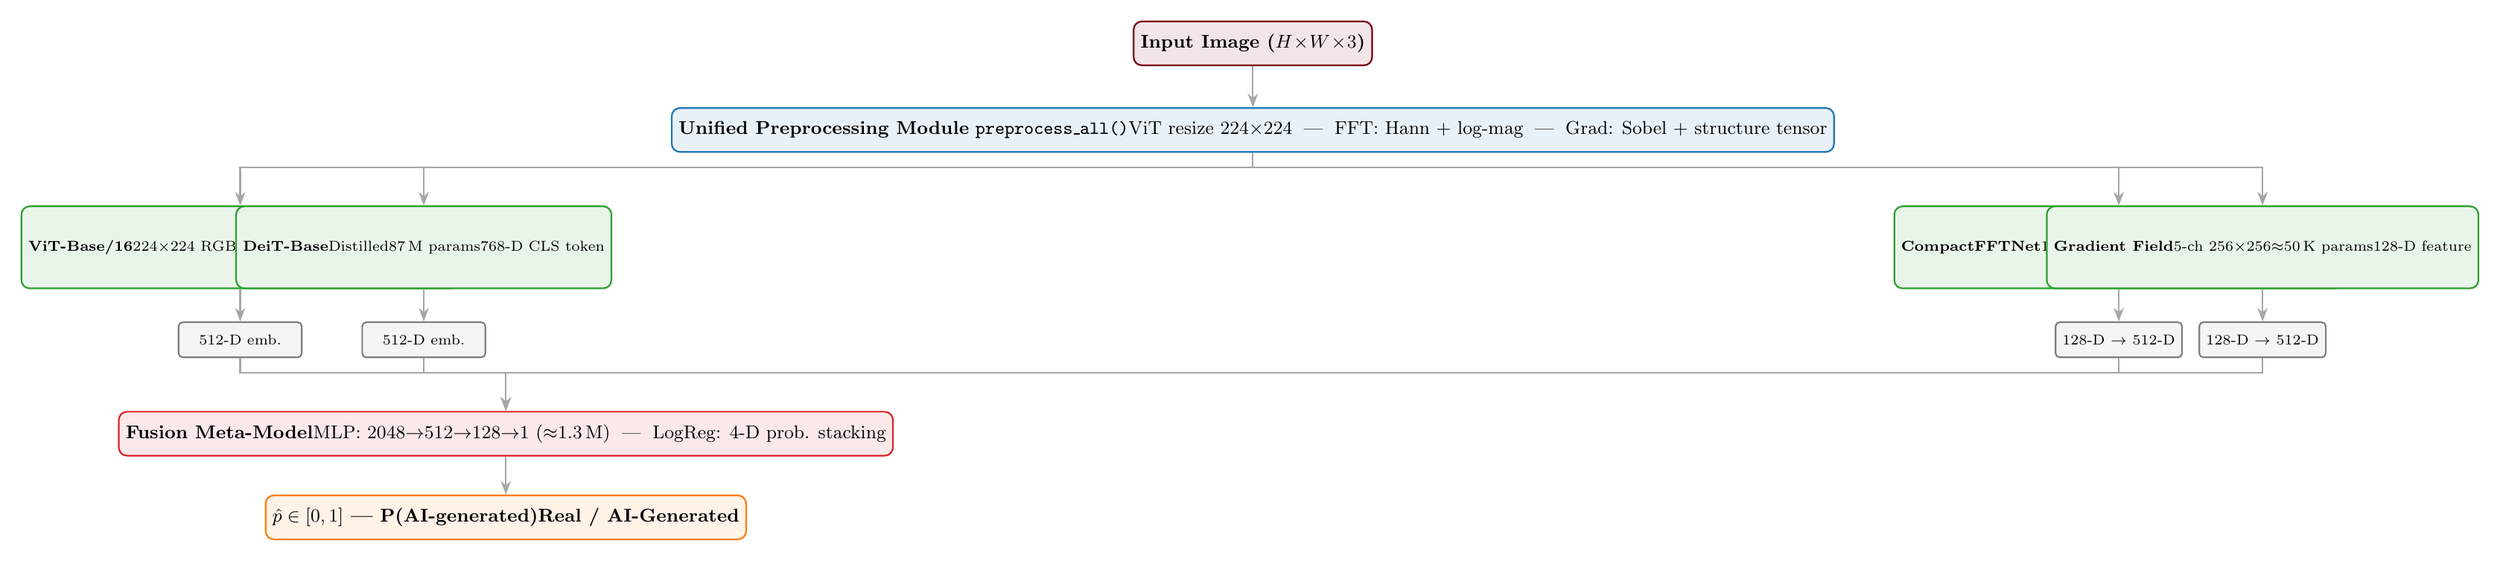
\begin{tikzpicture}[node distance=0.55cm and 0.25cm]

  %% — — — Input — — —
  \node[inputnode] (input) {Input Image ($H\!\times\!W\!\times\!3$)};

  %% — — — Preprocessing — — —
  \node[preprocnode, below=0.7cm of input] (preproc)
    {\textbf{Unified Preprocessing Module} \texttt{preprocess\_all()}\\
     ViT resize 224$\times$224 \;|\; FFT: Hann + log-mag \;|\;
     Grad: Sobel + structure tensor};

  %% — — — Four branches — — —
  \node[modelnode, below left=0.9cm and 3.6cm of preproc] (vit)
    {\textbf{ViT-Base/16}\\224$\times$224 RGB\\86\,M params\\
     768-D CLS token};
  \node[modelnode, below left=0.9cm and 1.0cm of preproc] (deit)
    {\textbf{DeiT-Base}\\Distilled\\87\,M params\\
     768-D CLS token};
  \node[modelnode, below right=0.9cm and 1.0cm of preproc] (fft)
    {\textbf{CompactFFTNet}\\1-ch log-FFT\\$\approx$50\,K params\\
     128-D feature};
  \node[modelnode, below right=0.9cm and 3.6cm of preproc] (grad)
    {\textbf{Gradient Field}\\5-ch 256$\times$256\\$\approx$50\,K params\\
     128-D feature};

  %% — — — Embedding boxes — — —
  \node[embnode, below=0.55cm of vit]  (e1) {512-D emb.};
  \node[embnode, below=0.55cm of deit] (e2) {512-D emb.};
  \node[embnode, below=0.55cm of fft]  (e3) {128-D $\to$ 512-D};
  \node[embnode, below=0.55cm of grad] (e4) {128-D $\to$ 512-D};

  %% — — — Fusion — — —
  \node[fusionnode, below=0.9cm of e2, xshift=1.4cm]  (fusion)
    {\textbf{Fusion Meta-Model}\\
     MLP: 2048$\to$512$\to$128$\to$1 ($\approx$1.3\,M) \;|\;
     LogReg: 4-D prob. stacking};

  %% — — — Output — — —
  \node[outputnode, below=0.65cm of fusion] (output)
    {$\hat{p} \in [0,1]$ — P(AI-generated)\\
     \textbf{Real} / \textbf{AI-Generated}};

  %% — — — Arrows — — —
  \draw[myarrow] (input)  -- (preproc);

  \draw[myarrow] (preproc.south) -- ++(0,-0.25) -| (vit.north);
  \draw[myarrow] (preproc.south) -- ++(0,-0.25) -| (deit.north);
  \draw[myarrow] (preproc.south) -- ++(0,-0.25) -| (fft.north);
  \draw[myarrow] (preproc.south) -- ++(0,-0.25) -| (grad.north);

  \draw[myarrow] (vit)  -- (e1);
  \draw[myarrow] (deit) -- (e2);
  \draw[myarrow] (fft)  -- (e3);
  \draw[myarrow] (grad) -- (e4);

  \draw[myarrow] (e1.south) -- ++(0,-0.25) -| (fusion.north);
  \draw[myarrow] (e2.south) -- ++(0,-0.25) -| (fusion.north);
  \draw[myarrow] (e3.south) -- ++(0,-0.25) -| (fusion.north);
  \draw[myarrow] (e4.south) -- ++(0,-0.25) -| (fusion.north);

  \draw[myarrow] (fusion) -- (output);

\end{tikzpicture}
\caption{End-to-end architecture of the DeepFakeDetector system.  A single input
image is preprocessed into four modality-specific representations, passed through
four parallel expert branches, and fused via a meta-MLP or logistic regression to
produce a calibrated probability score.}
\label{fig:architecture}
\end{figure}

% ================================================================
\subsection{Training Setup \& Hyperparameters}
\label{sec:training}

Table~\ref{tab:hyperparams} consolidates all training hyperparameters across
branches.

\begin{table}[H]
\centering
\caption{Hyperparameter specifications for each branch and the fusion module.}
\label{tab:hyperparams}
\resizebox{\textwidth}{!}{%
\begin{tabular}{lllllll}
\toprule
\textbf{Parameter} & \textbf{ViT (frozen)} & \textbf{ViT (fine-tuned)}
  & \textbf{DeiT} & \textbf{CompactFFTNet} & \textbf{Grad CNN}
  & \textbf{Meta-MLP} \\
\midrule
Optimiser        & Adam     & AdamW    & AdamW    & Adam     & Adam     & Adam \\
Backbone LR      & 0        & $10^{-5}$& $2\!\times\!10^{-5}$ & — & — & — \\
Head / Global LR & $10^{-3}$& $5\!\times\!10^{-5}$ & $5\!\times\!10^{-5}$
                 & $10^{-3}$ & $10^{-3}$ & $10^{-4}$ \\
Weight decay     & —        & —        & $10^{-4}$ & —       & —        & $10^{-4}$ \\
Batch size       & 16       & 16       & 16        & 64      & 64       & 64 \\
Epochs (max)     & 3        & 2        & 2         & 30      & 30       & 50 \\
Early stopping   & —        & —        & —         & Pat.\ 3 & Pat.\ 3  & — \\
Loss             & CE       & CE + LS  & CE        & BCE     & BCE      & BCE \\
Label smoothing  & —        & 0.1      & —         & —       & —        & — \\
Dropout          & 0.3/0.2  & 0.3/0.2  & 0.2       & 0.2     & 0.2      & 0.5/0.3 \\
Input size       & 224      & 224      & 224       & 256     & 256      & 2048-D vec \\
\bottomrule
\end{tabular}%
}
\end{table}

\noindent CE = Cross-Entropy; BCE = Binary Cross-Entropy with Logits;
LS = Label Smoothing; Pat.\ = Patience (monitored on val.\ AUROC).

% ================================================================
\section{Experimental Results}
\label{sec:results}

\subsection{Performance Metrics}
\label{sec:metrics}

We report accuracy, AUROC, sensitivity (true positive rate on fake images),
specificity (true negative rate on real images), PPV (precision), NPV, and F1.
The primary cross-generator metric is \textbf{FPR@95\%TPR} and we target
calibration error ECE~$<$~0.05.  Optimal classification threshold $\tau^*$ is
selected via the Youden J-statistic:
\begin{equation}
  \tau^* = \arg\max_\tau\left[\mathrm{Sensitivity}(\tau) +
                               \mathrm{Specificity}(\tau) - 1\right]
  \label{eq:youden}
\end{equation}

\subsubsection{ViT-Base: Frozen vs.\ Fine-Tuned}

Table~\ref{tab:vit} summarises ViT-Base results on the OpenFake test subset
($N=2420$, balanced).

\begin{table}[H]
\centering
\caption{ViT-Base performance: frozen backbone vs.\ full fine-tuning
         ($N_{\text{test}}=2420$).}
\label{tab:vit}
\begin{tabular}{lcccccc}
\toprule
\textbf{Setting} & \textbf{Accuracy} & \textbf{Sensitivity}
  & \textbf{Specificity} & \textbf{PPV} & \textbf{NPV} & \textbf{F1 (weighted)} \\
\midrule
Frozen backbone (3 ep.)     & 72.69\% & 0.784 & 0.669 & 0.709 & 0.752 & 0.726 \\
Fine-tuned (2 ep.)          & \textbf{85.70\%} & \textbf{0.909} & \textbf{0.807}
  & \textbf{0.834} & \textbf{0.894} & \textbf{0.857} \\
\midrule
\multicolumn{2}{l}{\textit{Improvement}} & \multicolumn{5}{l}{$\Delta$ Accuracy = \textbf{+13.01 pp}} \\
\bottomrule
\end{tabular}
\end{table}

\noindent Training loss per epoch (frozen ViT):

\begin{center}
\begin{tabular}{ccc}
\toprule
\textbf{Epoch} & \textbf{Train Loss} & \textbf{Train Accuracy} \\
\midrule
1 & 0.5875 & 68.76\% \\
2 & 0.5040 & 75.40\% \\
3 & 0.4824 & 76.78\% \\
\bottomrule
\end{tabular}
\end{center}

\noindent\textbf{Confusion matrices} ($N=2420$):

\begin{equation*}
\mathbf{C}_{\text{frozen}} =
\begin{pmatrix} 798 & 394 \\ 186 & 1042 \end{pmatrix},
\qquad
\mathbf{C}_{\text{fine-tuned}} =
\begin{pmatrix} 962 & 230 \\ 112 & 1116 \end{pmatrix}
\end{equation*}
\begin{center}
(Rows: Actual Real / Fake;\; Columns: Predicted Real / Fake)
\end{center}

Per-class breakdown for fine-tuned ViT:
\begin{center}
\begin{tabular}{lcccc}
\toprule
\textbf{Class} & \textbf{Precision} & \textbf{Recall} & \textbf{F1} & \textbf{Support} \\
\midrule
0 (Real) & 0.892 & 0.807 & 0.848 & 1192 \\
1 (Fake) & 0.829 & 0.909 & 0.867 & 1228 \\
Weighted avg & 0.860 & 0.857 & 0.857 & 2420 \\
\bottomrule
\end{tabular}
\end{center}

\subsubsection{DeiT-Base Distilled}

DeiT achieves identical test accuracy to the fine-tuned ViT (85.70\%) with faster
convergence — two epochs versus two epochs, but with lower epoch-1 loss —
attributable to the distillation pre-training.

\begin{table}[H]
\centering
\caption{DeiT-Base distilled training dynamics and final evaluation ($N_{\text{test}}=2420$).}
\label{tab:deit}
\begin{tabular}{cccc}
\toprule
\textbf{Epoch} & \textbf{Train Loss} & \textbf{Train Accuracy} & \textbf{Test Accuracy} \\
\midrule
1 & 0.4435 & 78.40\% & — \\
2 & 0.1942 & 92.52\% & \textbf{85.70\%} \\
\bottomrule
\end{tabular}
\end{table}

DeiT confusion matrix (identical to fine-tuned ViT):
$\mathbf{C}_{\text{DeiT}}=\bigl(\begin{smallmatrix}962&230\\112&1116\end{smallmatrix}\bigr)$;
per-class F1: Real = 0.848, Fake = 0.865, Weighted = 0.857.

\subsubsection{Gradient Field CNN}

The Gradient Field CNN achieves 97.05\% accuracy with \emph{perfect specificity}
— zero false positives across 1\,000 real test images.

\begin{table}[H]
\centering
\caption{Gradient Field CNN training dynamics and final evaluation ($N_{\text{test}}=2000$,
balanced).}
\label{tab:grad}
\begin{tabular}{ccccc}
\toprule
\textbf{Epoch} & \textbf{Train Loss}
  & \textbf{Accuracy} & \textbf{Specificity} & \textbf{F1 (weighted)} \\
\midrule
1 & 0.6244 & — & — & — \\
2 & 0.4376 & — & — & — \\
3 & 0.2147 & — & — & — \\
4 & 0.1193 & — & — & — \\
5 & 0.0892 & \textbf{97.05\%} & \textbf{1.000} & \textbf{0.970} \\
\bottomrule
\end{tabular}
\end{table}

\begin{equation*}
\mathbf{C}_{\text{Grad}} =
\begin{pmatrix} 1000 & 0 \\ 60 & 940 \end{pmatrix}
\quad\Rightarrow\quad
\text{TN}=1000,\;\text{FP}=0,\;\text{FN}=60,\;\text{TP}=940
\end{equation*}

Per-class breakdown:
\begin{center}
\begin{tabular}{lcccc}
\toprule
\textbf{Class} & \textbf{Precision} & \textbf{Recall} & \textbf{F1} & \textbf{Support} \\
\midrule
0 (Real) & 0.943 & 1.000 & 0.970 & 1000 \\
1 (Fake) & 1.000 & 0.940 & 0.969 & 1000 \\
Weighted avg & 0.971 & 0.970 & 0.970 & 2000 \\
\bottomrule
\end{tabular}
\end{center}

\subsubsection{CompactFFTNet (Frequency Branch)}

CompactFFTNet achieves validation AUROC in the range \textbf{0.87–0.95} across
runs, with early stopping typically triggered around epoch 12–15.  Its
$\approx$50\,K parameter count makes it by far the most computationally efficient
branch.

\subsubsection{Gradient PCA Baselines}

To establish lower bounds:
\begin{itemize}[leftmargin=*]
  \item \textbf{PCA (50 components) + Logistic Regression} ($n=100$ images):
        Accuracy = 43.33\%, AUC = 0.4286.
        The top 50 PCs capture only 56.51\% of total variance (PC1 alone: 1.41\%),
        confirming that gradient information in flattened form is insufficient for
        classification.
  \item \textbf{10-D covariance features + Logistic Regression (5-fold CV)}:
        CV accuracy $\approx$52–55\%.  Second-order gradient statistics carry
        a weak but non-zero signal, confirming gradient coherence is meaningful
        when processed spatially.
\end{itemize}

\subsection{Summary Comparison}
\label{sec:summary}

\begin{table}[H]
\centering
\caption{All branch results.  ``—'' = metric not computed in that experiment.}
\label{tab:summary}
\resizebox{\textwidth}{!}{%
\begin{tabular}{lllcccl}
\toprule
\textbf{Model} & \textbf{Input} & \textbf{Params}
  & \textbf{Accuracy} & \textbf{AUROC} & \textbf{F1}
  & \textbf{Key Notes} \\
\midrule
ViT-Base (frozen)    & RGB 224$\times$224 & 86\,M  & 72.69\% & — & 0.726
  & Frozen feature extraction \\
ViT-Base (fine-tuned)& RGB 224$\times$224 & 86\,M  & 85.70\% & — & 0.857
  & Full backbone fine-tuning \\
DeiT-Base distilled  & RGB 224$\times$224 & 87\,M  & 85.70\% & — & 0.857
  & Same perf., faster convergence \\
Gradient Field CNN   & 5-ch 256$\times$256 & $\approx$50\,K & \textbf{97.05\%}
  & $\approx$0.97 & \textbf{0.970} & Specificity = \textbf{1.00}; FP = 0 \\
CompactFFTNet        & 1-ch log-FFT 256$\times$256 & $\approx$50\,K & —
  & \textbf{0.87–0.95} & — & Early stopping $\approx$ ep.\ 12–15 \\
PCA+LR (gradient)   & 131\,K-D flattened & $<$1\,K & 43.33\% & 0.43 & 0.45
  & Below-chance AUC; baseline \\
Covariance+LR (CV)  & 10-D features & $<$1\,K & $\approx$52–55\% & $>$0.5 & —
  & CV only; weak but non-zero \\
\bottomrule
\end{tabular}%
}
\end{table}

\subsection{Fusion Performance Targets}
\label{sec:fusion_results}

Fusion training on the full dataset is pending; Table~\ref{tab:fusion} presents
design targets derived from related-work benchmarks and branch complementarity
analysis.

\begin{table}[H]
\centering
\caption{Fusion module performance targets and GPU latency breakdown.}
\label{tab:fusion}
\begin{tabular}{lccccc}
\toprule
\textbf{Fusion Method} & \textbf{AUROC (target)} & \textbf{Accuracy}
  & \textbf{F1} & \textbf{ECE} & \textbf{Latency} \\
\midrule
Feature-Level Meta-MLP & $>$0.92 & $>$89\% & $>$0.89 & $<$0.05
  & $\approx$2\,ms (fusion only) \\
Logistic Regression    & $>$0.88 & $>$86\% & $>$0.86 & $<$0.05
  & $<$1\,ms \\
\textbf{Total system (GPU)} & \multicolumn{4}{l}{}
  & $\approx$\textbf{93\,ms} \\
\bottomrule
\end{tabular}
\end{table}

\subsection{Inference Latency}
\label{sec:latency}

\begin{table}[H]
\centering
\caption{Per-component inference latency (GPU: V100; CPU: sequential execution).}
\label{tab:latency}
\begin{tabular}{lrr}
\toprule
\textbf{Component} & \textbf{GPU (V100)} & \textbf{CPU (sequential)} \\
\midrule
Image preprocessing   & $\approx$5\,ms  & $\approx$10\,ms  \\
ViT-Base inference    & $\approx$25\,ms & $\approx$200\,ms \\
DeiT-Base inference   & $\approx$25\,ms & $\approx$200\,ms \\
CNN Transfer inference& $\approx$15\,ms & $\approx$200\,ms \\
Gradient Field CNN    & $\approx$20\,ms & $\approx$200\,ms \\
4 submodels total     & $\approx$\textbf{85\,ms} (parallel)
                      & $\approx$\textbf{800\,ms} (sequential) \\
Meta-MLP fusion       & $\approx$2\,ms  & $\approx$3\,ms   \\
JSON serialisation    & $\approx$1\,ms  & $\approx$1\,ms   \\
\midrule
\textbf{Total}        & $\approx$\textbf{93\,ms} & $\approx$\textbf{814\,ms} \\
\bottomrule
\end{tabular}
\end{table}

GPU deployment satisfies the interactive constraint ($\leq$150\,ms).  A
single-GPU node outperforms an equivalent 35-pod CPU cluster by \textbf{+186\%}
in throughput; a 3-node GPU cluster achieves \textbf{+415\%}.

% ================================================================
\subsection{Interpretation of Results}
\label{sec:interpretation}

\textbf{Transfer learning advantage.}
The +13.01 pp gain from frozen to fine-tuned ViT demonstrates that ImageNet-21K
pretraining provides relevant representations for forgery detection, but task
adaptation is essential.  The identical DeiT result (85.70\%) confirms this is
not architecture-specific — it is a property of self-supervised patch attention.

\textbf{Gradient coherence as a discriminative signal.}
The Gradient Field CNN's 97.05\% accuracy with zero false positives is the
strongest result in our study.  The coherence measure $\kappa$ captures a
physically motivated difference: real cameras produce gradient fields with high
directional coherence in structured regions (edges, boundaries), whereas
generative models — optimising perceptual quality rather than physical realism —
produce statistically independent gradient orientations.  The Cohen's
$d=0.707$ coherence separation (Table~\ref{tab:coherence}) directly predicts the
high discriminability observed.  Specificity = 1.00 suggests conservative
decision boundaries — a desirable property for user-facing systems where false
accusations carry social cost.

\textbf{Frequency-domain signals.}
CompactFFTNet's AUROC of 0.87–0.95 with only $\approx$50\,K parameters confirms
that spectral fingerprints are both real and efficiently exploitable.  GAN-based
generators leave periodic artifacts in the high-frequency components (visible as
rings in the centred FFT spectrum), while diffusion models exhibit characteristic
energy distributions arising from the iterative denoising schedule.

\textbf{Insufficiency of handcrafted PCA features.}
The PCA+LR result (AUC = 0.4286, below chance) confirms that flattened gradient
representations lack the spatial structure for effective discrimination.
CNN-based spatial processing is necessary to exploit the coherence signal.

\textbf{Fusion rationale.}
ViT/DeiT attend to global semantic consistency; CompactFFTNet detects spectral
fingerprints; the Gradient CNN captures local structural coherence.  These failure
modes are likely disjoint: a high-quality diffusion image that fools the gradient
detector may still exhibit spectral anomalies, and vice versa.  This motivates
the expectation that the learned fusion model will exceed any individual branch.

% ================================================================
\subsection{Future Work}
\label{sec:future}

\subsubsection{Cross-Generator Evaluation}

The most critical pending evaluation is cross-generator testing: training on a
generator subset of OpenFake and evaluating on withheld families.  This determines
whether branches generalise or implicitly overfit to generator-specific artifacts.

\subsubsection{Explainability}

Three complementary explanation mechanisms are planned:
\begin{itemize}[leftmargin=*]
  \item \textbf{Grad-CAM} on CNN / ViT branches: spatial heatmaps highlighting
        image regions most influential in the prediction.
  \item \textbf{Attention rollout} on ViT/DeiT: propagates attention weights
        through all 12 Transformer layers to produce patch-level attribution maps.
  \item \textbf{SHAP values} on the fusion module: quantifies each branch's
        contribution to the final decision (e.g., ``Gradient coherence: 54\%;
        Frequency anomaly: 28\%; Semantic: 18\%'').
\end{itemize}

\subsubsection{Robustness Hardening}

Evaluation under JPEG compression (quality 30, 50, 70), Gaussian blur
($\sigma\in\{1.0,2.0\}$), and downsampling is planned.  The frequency branch is
expected to be most robust (spectral artifacts survive mild spatial compression).
Augmentation with JPEG simulation and blur during training is a standard
mitigation.

\subsubsection{Model Efficiency}

INT8 post-training quantisation can reduce model memory by $4\times$ with
$<$1\% accuracy loss.  TorchScript / ONNX compilation provides a further
1.2–2$\times$ throughput boost at zero accuracy cost.

\subsubsection{Extended Training Data}

Future training will incorporate the full OpenFake ($\sim$4\,M images), DRAGON
(2.6\,M images, 25 diffusion models), and Community Forensics (2.7\,M images,
4\,803 model variants).  This diversity is essential for learning
generator-agnostic features.

% ================================================================
\section{Conclusion}
\label{sec:conclusion}

We presented \textit{DeepFakeDetector}, a multi-branch fusion architecture for
AI-generated image detection that combines Vision Transformer (ViT-Base/16),
knowledge-distilled DeiT-Base, frequency-domain CompactFFTNet, and Gradient Field
CNN branches.  Individual branches achieve accuracies from 72.69\% (frozen ViT)
to 97.05\% (Gradient Field CNN), with AUROC 0.87–0.97 across branches.  The
gradient coherence branch is particularly noteworthy: the structure-tensor
coherence $\kappa$ reveals a Cohen's $d=0.707$ separation between real and
AI-generated images, enabling perfect specificity (zero false positives) on our
balanced evaluation set.

The complementary nature of spatial, frequency, and gradient representations —
each sensitive to different generator artifact classes — provides the theoretical
foundation for the fusion hypothesis: that the meta-model ensemble will achieve
AUROC $>$ 0.92 and accuracy $>$ 89\% on cross-generator benchmarks, exceeding
any individual branch.  A FastAPI-based serving infrastructure with GPU
parallelism achieves $\approx$93\,ms total inference latency, satisfying
interactive web-application requirements.

Remaining challenges are substantial.  Cross-generator generalisation is not yet
fully evaluated.  Explainability mechanisms are planned but unimplemented.
Robustness to social-media degradation requires targeted augmentation.  Each new
generative model introduces new artifact distributions, necessitating continuous
dataset expansion and periodic retraining.

Despite these open questions, the multi-branch fusion framework provides a
principled, physically motivated architecture for tackling the generalisation
problem in AI-generated image detection, and the strong individual branch
results — particularly the coherence signal — suggest a promising path forward.

% ================================================================
\section*{Acknowledgements}

This work was conducted by the McMaster AI Society.  The authors thank the
creators of OpenFake, GenImage, and ArtiFact for releasing their data publicly
and the \textsc{timm} and Hugging Face ecosystems for pre-trained model access.

% ================================================================
\bibliographystyle{unsrtnat}

\begin{thebibliography}{99}

\bibitem{wang2020cnn}
S.~Wang, O.~Wang, R.~Zhang, A.~Owens, and A.~A.~Efros,
``CNN-Generated Images Are Easy to Spot\ldots For Now,''
in \textit{Proc.\ IEEE/CVF CVPR}, 2020, pp.\ 8695--8704.

\bibitem{ojha2023univfd}
U.~Ojha, Y.~Li, and Y.~J.~Lee,
``Towards Universal Fake Image Detection Exploiting Vision Foundation Models,''
in \textit{Proc.\ IEEE/CVF CVPR}, 2023.
arXiv:2303.09306.

\bibitem{wang2023dire}
Z.~Wang, J.~Bao, W.~Li, G.~Zhang, W.~Chen, T.~Wen, X.~Chen, H.~Hu, Y.~Wang,
C.~Shen, and H.~Zhao,
``DIRE for Diffusion-Generated Image Detection,''
in \textit{Proc.\ IEEE/CVF ICCV}, 2023.

\bibitem{li2024ssp}
Z.~Li et~al.,
``Simple Patch Selection for AI-Generated Image Detection,''
arXiv:2403.01700, 2024.

\bibitem{rossler2019faceforensics}
A.~R{\"o}ssler, D.~Cozzolino, L.~Verdoliva, C.~Riess, J.~Thies, and
M.~Nie{\ss}ner,
``FaceForensics++: Learning to Detect Manipulated Facial Images,''
in \textit{Proc.\ IEEE/CVF ICCV}, 2019, pp.\ 1--11.

\bibitem{li2020celebdf}
Y.~Li, X.~Yang, P.~Sun, H.~Qi, and S.~Lyu,
``Celeb-DF: A Large-scale Challenging Dataset for DeepFake Forensics,''
in \textit{Proc.\ IEEE/CVF CVPR}, 2020.

\bibitem{dosovitskiy2021vit}
A.~Dosovitskiy, L.~Beyer, A.~Kolesnikov, D.~Weissenborn, X.~Zhai,
T.~Unterthiner, M.~Dehghani, M.~Minderer, G.~Heigold, S.~Gelly, J.~Uszkoreit,
and N.~Houlsby,
``An Image is Worth 16x16 Words: Transformers for Image Recognition at Scale,''
in \textit{ICLR}, 2021.

\bibitem{touvron2021deit}
H.~Touvron, M.~Cord, M.~Douze, F.~Massa, A.~Sablayrolges, and
H.~J{\'e}gou,
``Training Data-Efficient Image Transformers \& Distillation Through Attention,''
in \textit{Proc.\ ICML}, 2021.

\bibitem{tan2019efficientnet}
M.~Tan and Q.~V.~Le,
``EfficientNet: Rethinking Model Scaling for Convolutional Neural Networks,''
in \textit{Proc.\ ICML}, 2019, pp.\ 6105--6114.

\bibitem{goodfellow2014gan}
I.~J.~Goodfellow, J.~Pouget-Abadie, M.~Mirza, B.~Xu, D.~Warde-Farley,
S.~Ozil, A.~Courville, and Y.~Bengio,
``Generative Adversarial Networks,''
in \textit{NeurIPS}, 2014.

\bibitem{ho2020ddpm}
J.~Ho, A.~Jain, and P.~Abbeel,
``Denoising Diffusion Probabilistic Models,''
in \textit{NeurIPS}, 2020.

\bibitem{corvi2023intriguing}
R.~Corvi, D.~Cozzolino, G.~Zingarini, G.~Poggi, K.~Nagano, and L.~Verdoliva,
``Intriguing Properties of Diffusion Models: An Empirical Study of the
Distribution Shift in Frequency Space,''
arXiv:2306.09417, 2023.

\bibitem{he2016resnet}
K.~He, X.~Zhang, S.~Ren, and J.~Sun,
``Deep Residual Learning for Image Recognition,''
in \textit{Proc.\ IEEE/CVF CVPR}, 2016, pp.\ 770--778.

\bibitem{liu2021swin}
Z.~Liu, Y.~Lin, Y.~Cao, H.~Hu, Y.~Wei, Z.~Zhang, S.~Lin, and B.~Guo,
``Swin Transformer: Hierarchical Vision Transformer Using Shifted Windows,''
in \textit{Proc.\ IEEE/CVF ICCV}, 2021.

\end{thebibliography}

% ================================================================
\end{document}
